% !TeX spellcheck = en_GB
\documentclass{beamer}\mode<presentation>{\usetheme{AMSCesenaPurpleAndGold}}
%\documentclass[presentation]{beamer}\mode<presentation>{\usetheme{AMSCesenaPurpleAndGold}}
%%%%

\usepackage{sd-lab-async-programming}
%\usepackage{my-listings}

\newcommand{\labN}{3}
\newcommand{\labGroup}{https://gitlab.com/pika-lab/courses/ds/ay2021}
\newcommand{\labRepo}{\labGroup/lab-\labN}

\title[L\labN{} -- Async Programming 101]{L\labN{} -- Asynchronous Programming 101}
%
\subtitle[SD]{Distributed Systems\\\scriptsize Technologies}
%
\author[Ciatto \and Omicini]
{\emph{Giovanni Ciatto} \and Andrea Omicini\\
	\texttt{giovanni.ciatto@unibo.it \and andrea.omicini@unibo.it}}
%
\institute[DISI, Univ. Bologna]
{Dipartimento di Informatica -- Scienza e Ingegneria (DISI)\\\textsc{Alma Mater Studiorum} -- Universit{\`a} di Bologna a Cesena}
%
\date[A.Y. 2020/2021]{Academic Year 2020/2021}

\setbeamercovered{transparent}

\AtBeginSection{
	\begin{frame}[c]\frametitle{Outline}
		% 		\begin{multicols}{2}
		\tableofcontents[sectionstyle=show/shaded, subsectionstyle=hide/hide, subsubsectionstyle=hide/hide]
		% 		\end{multicols}
	\end{frame}
}

\AtBeginSubsection{
	\begin{frame}[c]\frametitle{Next in Line\ldots}
		\begin{multicols}{2}
			\tableofcontents[sectionstyle=show/shaded, subsectionstyle=show/shaded, subsubsectionstyle=hide/hide]
		\end{multicols}
	\end{frame}
}

\begin{document}

%\\\\\\\\\\\\\\\\\\\\\
\frame{\titlepage}
%\\\\\\\\\\\\\\\\\\\\\

\section{Overview}

\begin{frame}
\frametitle{Motivation \& Lecture Goals}

\begin{itemize}
	\item Asynchronous programming is a fundamental paradigm for distributed or concurrent systems

	\vfill

	\item In particular in this course we need it to show how some mechanisms are achieved
	%
	\begin{itemize}
		\item e.g. \linda{}'s suspensive semantics
	\end{itemize}

	\vfill

	\item Furthermore, asynchronous programming is the \emph{de facto} standard for the development of real-world distributed applications

	\vfill

	\item For all such reasons, in this tutorial we introduce the notions of \alert{executor service}, \alert{future}, and \alert{promise} in Java
	%
	\begin{itemize}
		\item equivalent constructs exist in all mainstream languages nowadays
	\end{itemize}
\end{itemize}

\end{frame}

\begin{frame}
\frametitle{Lab \labN{} Repository on GitLab}

	\begin{itemize}
		\item Examples and exercises described in this lecture are provided by means of the following GitLab repository:
		%
		\begin{center}
			\url{\labRepo}
		\end{center}

		\vfill

		\item Clone it on your machine using Git
		%
		\begin{itemize}
		    \item[\$] \texttt{git clone \textit{<repo URL>}}
		\end{itemize}

		\vfill

		\item Even if a minimal environment simply relying on a text editor + Gradle is sufficient for this lab, we kindly suggest to import the cloned repository into some IDE, e.g. IntelliJ Idea or Eclipse

		\vfill

		\item In order to be able to submit your exercises, please ensure you requested access to the \href{\labGroup}{GitLab group of the course}
	\end{itemize}

\end{frame}

\section{Fundamentals}

\subsection{Executor Services}

\begin{frame}[allowframebreaks]\frametitle{Executor Services}

	\begin{itemize}
		\item Objects of type \href{https://docs.oracle.com/javase/8/docs/api/java/util/concurrent/ExecutorService.html}{\texttt{java.util.concurrent.\alert{ExecutorService}}} are useful for building \alert{concurrent} applications, abstracting threads away

		\bigskip

		\item An \alert{\texttt{ExecutorService}} is essentially a wrapper for one or more \alert{worker} threads + a \alert{task queue} which is consumed by such thread(s), where a task can be either:
		%
		\begin{itemize}
			\item an instance of \href{https://docs.oracle.com/javase/8/docs/api/java/lang/Runnable.html}{\texttt{java.lang.\alert{Runnable}}}, representing a \emph{procedure} to be \alert{executed} by the executor service

			\item an instances of \href{https://docs.oracle.com/javase/8/docs/api/java/util/concurrent/Callable.html}{\texttt{java.util.concurrent.\alert{Callable<X>}}}, representing a \emph{function}, returning type \texttt{X}, to be \alert{submitted} to the executor service
		\end{itemize}

		\bigskip

		\item Executor Services can be created by means of the \href{https://docs.oracle.com/javase/8/docs/api/java/util/concurrent/Executors.html}{\texttt{java.util.concurrent.Executor\alert{s}.new*()}} static methods
	\end{itemize}

	\framebreak

	\begin{center}
		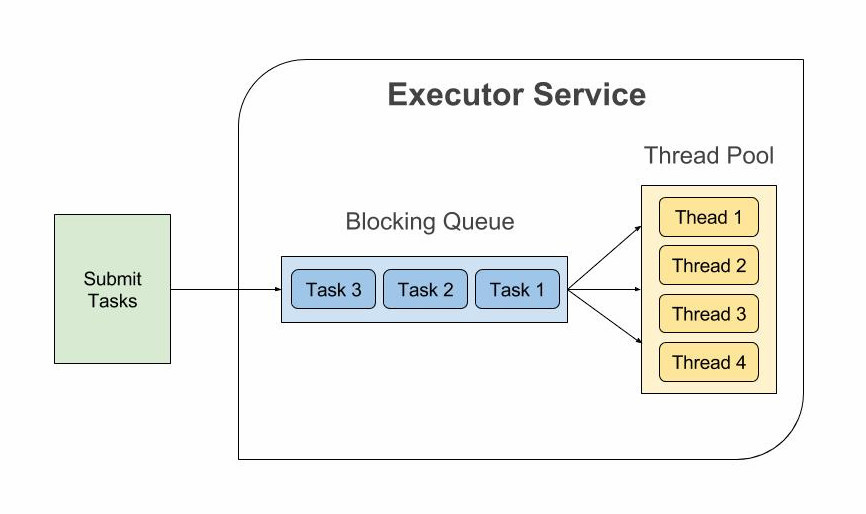
\includegraphics[width=.9\linewidth]{img/executor_service.jpg}

		{\tiny Source: \url{https://www.callicoder.com/java-executor-service-and-thread-pool-tutorial/}}
	\end{center}

	\framebreak

	\lstinputlisting[language=Java]{code/ExecutorService.java}

\end{frame}

\subsection{Runnables}

\begin{frame}[allowframebreaks]
\frametitle{Executing \texttt{Runnable}s -- Concept}

	\lstinputlisting[language=Java]{code/Runnable.java}

	\framebreak

	\begin{itemize}
		\item Runnables can be \alert{executed} on an executor service by means of its \texttt{void execute(Runnable task)} method
	\end{itemize}
	%
	\begin{center}
		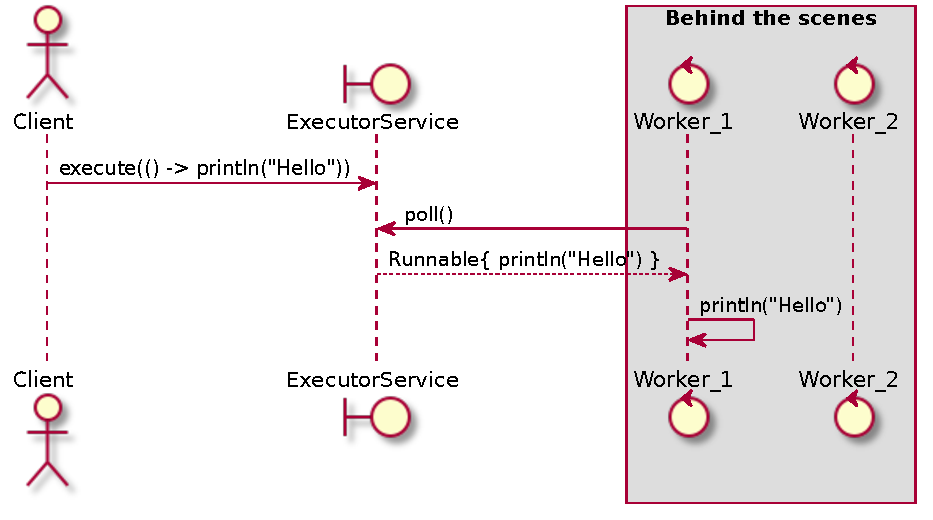
\includegraphics[width=.7\linewidth]{img/execute.pdf}
	\end{center}
	%
	\hint{When the \texttt{execute()} method returns, there is \alert{no guarantee} the task has \alert{already} been executed}

\end{frame}

\begin{frame}%[allowframebreaks]
\frametitle{Executing \texttt{Runnable}s -- Example}

	\lstinputlisting[language=Java]{./code/execute_example.java}

	\vfill

	\begin{itemize}
		\item \texttt{void shutdown()} prevents the executor service from accepting other tasks
	\end{itemize}

\end{frame}

\begin{frame}%[allowframebreaks]
\frametitle{More examples on \texttt{ExecutorService}s}

	Let's have a look to \texttt{sd.lab.concurrency.\alert{ExecutorServicesExamples}}

	\vfill

	\begin{block}{How to run a specific test in Gradle}
		\begin{itemize}
			\item[\$] \texttt{./gradlew cleanTest test --tests "full.package.of.\textit{TestClassName}.\alert{testMethodName}"}
		\end{itemize}
	\end{block}

	\vfill

	\begin{block}{How to interpret a test for concurrent/asynchronous code}
		If you need to test the interaction among \alert{concurrent} control flows:
		\begin{enumerate}
			\item create a shared, ordered data structure, e.g. \texttt{List<\alert{Integer}>}

			\item let the many control flows add items to the data structure

			\item wait for all control flows to terminate

			\item draw assertions on the items content \& ordering from within the data structure
		\end{enumerate}
	\end{block}

\end{frame}

\subsection{Splitting Recursive Computations}

\begin{frame}[allowframebreaks]
    \frametitle{Splitting long-lasting, \textbf{recursive} computations}

    \begin{itemize}
        \item \emph{Recursive} computations can be \alert{split} into several tasks
        %
        \begin{itemize}
            \item to be scheduled in a row
        \end{itemize}

        \bigskip

        \item Each task must do 2 things:
        %
        \begin{itemize}
            \item compute 1 step of the recursive algorithm
            \item schedule the execution of the next step (i.e. perform recursion)
        \end{itemize}

    \end{itemize}

    \bigskip

    \begin{block}{Advantages}
        \begin{itemize}
            \item No issues related to stack saturation
            %
            \begin{itemize}
                \item as tasks lay on the heap
            \end{itemize}

            \item The same executor service can carry on several algorithms
            %
            \begin{itemize}
                \item even if single-threaded
            \end{itemize}
        \end{itemize}
    \end{block}

    \bigskip

    \begin{exampleblock}{Recall that}
        \begin{itemize}
            \item Iteration and recursion are equivalent mechanisms
            \item Iterative algorithms can always be rewritten in recursive form (and vice-versa)
            \item Tail-recursive formulations should be preferred, if possible
        \end{itemize}
    \end{exampleblock}

    \framebreak

    Example:
    %
	\lstinputlisting[language=Java]{./code/AsyncCounter1.java}

    \framebreak

    Usage example:
    %
    \lstinputlisting[language=Java]{./code/singleActivity.java}
    %
    \begin{itemize}
        \item[!] have a look to \texttt{sd.lab.concurrency.\alert{TestAsyncCounter1}}
    \end{itemize}

    \framebreak

    Consider having a look to the following examples as well
    %
    \begin{itemize}
        \item[!] \texttt{sd.lab.concurrency.\alert{SplittingComputationsExamples}}
    \end{itemize}

    \framebreak

    \begin{alertblock}{Problem}\centering
        How can the client code know when an asynchronous computation is over?
    \end{alertblock}

\end{frame}

\subsection{Callables \& Futures}

\begin{frame}[allowframebreaks]
\frametitle{Executing \texttt{Callable}s -- Concept}

	\lstinputlisting[language=Java]{./code/Callable.java}

	\framebreak

	\begin{itemize}
		\item Callables can be \alert{submitted} on an executor service by means of its \texttt{Future<X> submit(Callable<X> task)} method

		\vspace{.5cm}

		% \begin{itemize}
		\item The result of the asynchronous invocation can be retrieved by the caller by means of the returned \texttt{Future<X>} object
		% \end{itemize}

		\vspace{.5cm}

		\item Futures represent \alert{placeholders} for results that will \emph{eventually} be(come) available
	\end{itemize}

	\framebreak

	\lstinputlisting[language=Java]{./code/Future.java}

	\begin{itemize}
		\item the blocking operation, i.e. \texttt{get}, is called \texttt{wait} or \texttt{\alert{await}} in other languages
		%
		\begin{itemize}
			\item and it is not always an instance method
		\end{itemize}
	\end{itemize}

	\framebreak

	\begin{columns}
		\begin{column}{.6\linewidth}
			\begin{center}
				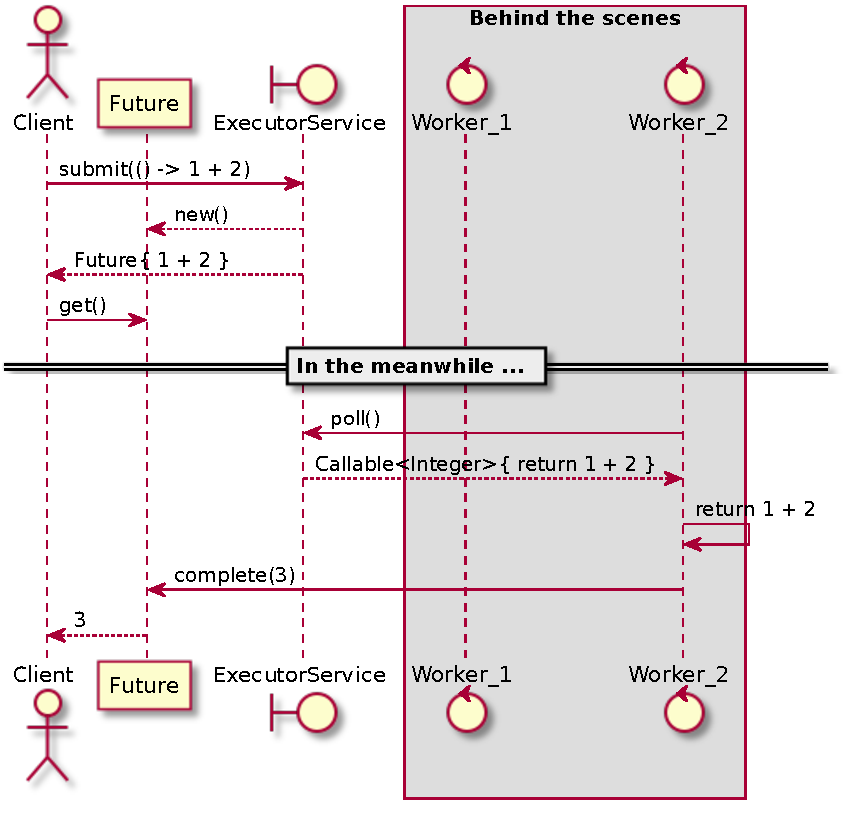
\includegraphics[width=\linewidth]{img/submit.pdf}
			\end{center}
		\end{column}
		\begin{column}{.4\linewidth}
			\begin{enumerate}
				\item The client \alert{submits} a callable to an executor service

				\item The executor service \alert{immediately} returns a future to the client

				\item To retrieve the result, the client must invoke the \alert{\texttt{Future::get}} method

				\item Such invocation \alert{blocks} until some worker thread \alert{comlpetes} the future with some result
			\end{enumerate}
		\end{column}
	\end{columns}

\end{frame}

\begin{frame}%[allowframebreaks]
\frametitle{Executing \texttt{Callables}s -- Example}

	\lstinputlisting[language=Java]{./code/submit_example.java}

\end{frame}

\begin{frame}[c]\frametitle{More examples on \texttt{Future}s}

	Consider having a look to the following examples as well
	%
	\begin{itemize}
		\item[!] \texttt{sd.lab.concurrency.\alert{FuturesExamples}}
	\end{itemize}

\end{frame}

\subsection{Promises}

\begin{frame}[allowframebreaks]
\frametitle{\texttt{CompletableFuture}s (a.k.a. Promises)}

	\begin{itemize}
		\item Futures are great for computing functions \alert{asynchronously}

		\medskip

		\item The examples presented so far, show how to create a future out of some Callable submission

		\medskip

		\item Can we explicitly decide which result should a future provide and when the caller should be unlocked?

		\bigskip

		\item[$\rightarrow$] \texttt{\alert{CompletableFuture}}s (or Promises) are what we need: they come with a \texttt{boolean complete(X value)} method which can be called within tasks
	\end{itemize}

	\framebreak

	\lstinputlisting[language=Java]{./code/CompletableFuture.java}

\end{frame}

\begin{frame}%[allowframebreaks]
\frametitle{\texttt{CompletableFuture}s (a.k.a. Promises) -- Example}

	\lstinputlisting[language=Java]{./code/AsyncCounter2.java}

\end{frame}

\begin{frame}%[allowframebreaks]
\frametitle{\texttt{CompletableFuture}s -- Client side}

	\lstinputlisting[language=Java]{./code/AsyncCounter2Test.java}

\end{frame}

\begin{frame}[c]
\frametitle{More examples on \texttt{CompletableFuture}s}

	Consider having a look to the following examples as well
	%
	\begin{itemize}
		\item[!] \texttt{sd.lab.concurrency.\alert{PromisesExamples}}
		\item[!] \texttt{sd.lab.concurrency.\alert{TestAsyncCounter2}}
	\end{itemize}

\end{frame}

\section{Check your understanding}

\startExercise

\subsection{Asynchronous Factorial Calculator}

\begin{frame}[c, allowframebreaks]
\frametitle{Exercise \currentExercise{} -- Asynchronous Factorial Calculator}

	Consider the interface \texttt{sd.lab.concurrency.exercise.\alert{AsyncFactorialCalculator}}:
	%
	\bigskip
	%
	\lstinputlisting[language=Java]{./code/AsyncCalculator.java}
	%
	\bigskip
	%
	\begin{enumerate}
		\item Provide an implementation for such an interface\ldots

		\bigskip

		\item \ldots in such a way that tests in \texttt{sd.lab\allowbreak{}.concurrency\allowbreak{}.exercise\allowbreak{}.\alert{TestAsyncCalculator}} are all satisfied

	\end{enumerate}

    \framebreak

	\begin{block}{Requirements}
		\begin{itemize}
			\item split the computation into multiple tasks
			\item exploit recursion \& promises
		\end{itemize}
	\end{block}

	\bigskip

    \begin{enumerate}\setcounter{enumi}{2}

		\item Submit your exercise to the following branch on Lab 3 repository
		%
		\begin{center}
			\texttt{submissions/\textit{name.surname}}
		\end{center}

		\bigskip

		\item Continuous Integration will automatically run tests
	\end{enumerate}

\end{frame}

\begin{frame}[c, allowframebreaks]
	\frametitle{Exercise \currentExercise{} -- Trivial Solution to be \textbf{Avoided}}

	Please \alert{avoid} the trivial solution where the whole computation is performed as a single task:
	%
	\lstinputlisting[language=Java]{./code/AsyncCalculatorWrong.java}

\end{frame}

\startExercise

\subsection{Custom Executor Service (Advanced)}

\begin{frame}[c, allowframebreaks]
	\frametitle{(Advanced) Exercise \currentExercise{} -- Custom Executor Service}

	\begin{alertblock}{This is an \textbf{advanced} exercise}
		\begin{itemize}
			\item feel free to skip it
			\item try it if you are curious about the idea of implementing your own executor service
		\end{itemize}
	\end{alertblock}

	\framebreak

	Consider the class \texttt{sd.lab.concurrency.exercise.\alert{SingleThreadedExecutorService}}: it consists of an \alert{incomplete} raw implementation of a \emph{single-threaded} executor service
	%
	\bigskip
	%
	\begin{enumerate}
		\item the goal of this exercise is to complete its implementation in such a way that tests in \texttt{sd.lab\allowbreak{}.concurrency\allowbreak{}.exercise\allowbreak{}.\alert{TestSingleThreadedExecutorService}}
		are all satisfied

		\bigskip

		\item to do so, your implementation should adhere to Java's \href{https://docs.oracle.com/javase/8/docs/api/java/util/concurrent/ExecutorService.html}{\texttt{ExecutorService} interface}
		%
		\begin{itemize}
			\item in all its methods, except the \texttt{invoke*} ones which lay outside the scope of this exercise
		\end{itemize}

		\bigskip

		\item consider reading the Javadoc of the following types and exploit them in your solution:
		%
		\begin{itemize}
			\item \href{https://docs.oracle.com/javase/8/docs/api/java/util/concurrent/ExecutorService.html}{\texttt{java.util.concurrent.ExecutorService}}
			\item \href{https://docs.oracle.com/javase/8/docs/api/java/util/concurrent/BlockingQueue.html}{\texttt{java.util.concurrent.BlockingQueue}}
			\item \href{https://docs.oracle.com/javase/8/docs/api/java/util/concurrent/LinkedBlockingDeque.html}{\texttt{java.util.concurrent.LinkedBlockingDeque}}
			\item \href{https://docs.oracle.com/javase/8/docs/api/java/lang/Thread.html}{\texttt{java.lang.Thread}}
		\end{itemize}

        \bigskip

        \item recall to un-ignore tests

        \bigskip

        \item submit your exercise to the following branch on Lab 3 repository
        %
        \begin{center}
            \texttt{submissions/\textit{name.surname}}
        \end{center}

        \bigskip

        \item Continuous Integration will automatically run tests

	\end{enumerate}

\end{frame}

%===============================================================================
\section*{}
%===============================================================================

%\\\\\\\\\\\\\\\\\\\\\
\frame{\titlepage}
%\\\\\\\\\\\\\\\\\\\\\

%%===============================================================================
%\section*{\refname}
%%===============================================================================
%
%%\\\\\\\\\\\\\\\\\\\\\
%%%%%
%%\begin{frame}[t,allowframebreaks]\scriptsize
%\begin{frame}[c]\footnotesize
%\frametitle{\refname}
%\bibliographystyle{apalike}
%\bibliography{sd-lab-async-programming}
%\end{frame}
%%\\\\\\\\\\\\\\\\\\\\\

%%%%%%%%%%%%%%%%%%%%%%%%%%%%%%%%%%%%%%%%%%%%%%%%%%%%%%%%%%%%%%%%%%%%%%%%%%%%%%%
\end{document}
%%%%%%%%%%%%%%%%%%%%%%%%%%%%%%%%%%%%%%%%%%%%%%%%%%%%%%%%%%%%%%%%%%%%%%%%%%%%%%%%

